\documentclass[11pt]{article}

% -------------------------
% Packages
% -------------------------
\usepackage[margin=1in]{geometry}
\usepackage{xcolor}
\usepackage{amsmath, amssymb}
\usepackage{graphicx}
\usepackage{array}
\usepackage{enumitem}
\usepackage{hyperref}
\usepackage{tikz}
\usetikzlibrary{arrows.meta, positioning, shapes.geometric, calc}

% -------------------------
% Colors (black/blue/red)
% -------------------------
\definecolor{myblue}{RGB}{0,70,160}
\definecolor{myred}{RGB}{180,30,40}

\hypersetup{
  colorlinks=true,
  linkcolor=myblue,
  urlcolor=myblue,
  citecolor=myblue
}

% -------------------------
% Simple styling helpers
% -------------------------
\newcommand{\blue}[1]{\textcolor{myblue}{#1}}
\newcommand{\red}[1]{\textcolor{myred}{#1}}

% FIX: use \dimexpr ... \relax for length arithmetic
\newenvironment{bluebox}
{\vspace{6pt}\noindent\begin{tikzpicture}
\node[
  draw=myblue, line width=1pt, rounded corners=8pt,
  inner sep=8pt,
  text width=\dimexpr\linewidth-18pt\relax
] (box) \bgroup
\begin{minipage}{\dimexpr\linewidth-32pt\relax}
\blue{\textbf{Key idea}}\par\vspace{4pt}}
{\end{minipage}\egroup;
\end{tikzpicture}\vspace{6pt}}

\newenvironment{redbox}
{\vspace{6pt}\noindent\begin{tikzpicture}
\node[
  draw=myred, line width=1pt, rounded corners=8pt,
  inner sep=8pt,
  text width=\dimexpr\linewidth-18pt\relax
] (box) \bgroup
\begin{minipage}{\dimexpr\linewidth-32pt\relax}
\red{\textbf{Watch out / Important}}\par\vspace{4pt}}
{\end{minipage}\egroup;
\end{tikzpicture}\vspace{6pt}}

\setlist[itemize]{topsep=3pt, itemsep=2pt}
\setlist[enumerate]{topsep=3pt, itemsep=2pt}

\title{\textbf{GPU Architecture + CUDA Notes}}
\author{Ananya Pagadala}
\date{}

\begin{document}
\maketitle

% ============================================================
\section{\blue{TFLOPS, Cores, and Performance (car count + speed analogy)}}

\textbf{Think of car count + speed} $\Rightarrow$ \fbox{\textbf{TFLOPS}}\\
\quad $\Rightarrow$ cores execute instructions in one cycle (think parallel processing)

\begin{redbox}
\textbf{But number of cores doesn't mean better performance.}\\
You need more context because cycle speed can differ in the GPU w/ more cores.
\end{redbox}

\textbf{Two knobs you were thinking about:}
\begin{enumerate}
\item \textbf{The car count} $\Rightarrow$ \textbf{core count}
\item \textbf{Core speed} $\Rightarrow$ clock / frequency
\end{enumerate}
\quad \textbf{TFLOPS is derived} from these (plus how many FLOPs per instruction).

\begin{bluebox}
\textbf{Memory recall shortcut:}\\
\textbf{TFLOPS} $\approx$ \textit{(cores)} $\times$ \textit{(clock)} $\times$ \textit{(FLOPs per cycle)}.
\end{bluebox}

So higher speed + core count means more energy consumption.\\
So even if a GPU has $\uparrow$ energy consumption, even if it has higher perf,
some company might opt for one with \textbf{$\downarrow$ perf/watt}.

\subsection*{\blue{Table: Why “more cores” isn’t always faster}}
\begin{center}
\renewcommand{\arraystretch}{1.15}
\begin{tabular}{|>{\bfseries}p{0.22\linewidth}|p{0.36\linewidth}|p{0.36\linewidth}|}
\hline
Factor & What it means & Why it can bottleneck \\
\hline
Core count & How many lanes of compute & More lanes don't help if traffic (memory) is slow \\
\hline
Clock speed & How fast lanes run & Higher clock can raise power/heat and throttle \\
\hline
Memory bandwidth & Bytes/sec from HBM/DRAM & If data can't feed cores, cores sit idle \\
\hline
Latency hiding & Extra warps ready to run & If not enough warps, stalls show up \\
\hline
Tensor cores & Special matrix units & Huge speedups only when workload matches (GEMM/conv) \\
\hline
\end{tabular}
\end{center}

\subsection*{\blue{You wrote: New features (supporting new data types) $\rightarrow$ tensor cores}}
So perf impacted by:
\begin{enumerate}
\item memory bandwidth
\item TFLOPS
\item tensor cores
\end{enumerate}

% ============================================================
\section{\blue{Data Types + Sizes (different ways to store numeric values)}}

\subsection*{\blue{Your sketch: ints + floats by bit-width}}
\begin{center}
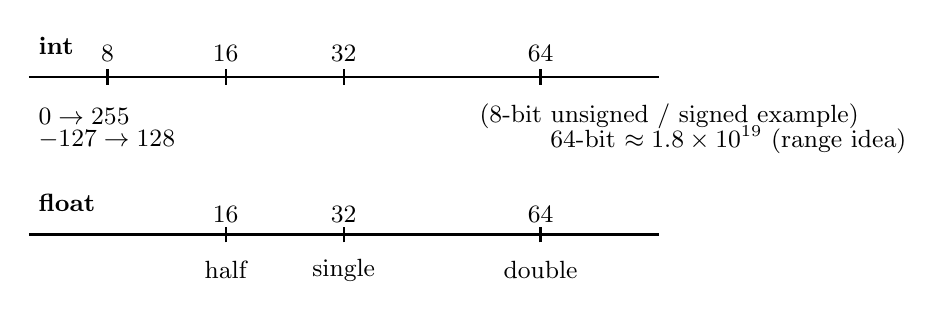
\begin{tikzpicture}[x=1cm,y=1cm, font=\small]
% INT timeline
\node[anchor=west] at (0,2) {\textbf{int}};
\draw[thick] (0,1.6) -- (8,1.6);
\foreach \x/\lab in {1/8, 2.5/16, 4/32, 6.5/64} {
  \draw[thick] (\x,1.5) -- (\x,1.7);
  \node at (\x,1.9) {\lab};
}
\node[anchor=west] at (0,1.1) {$0 \rightarrow 255$};
\node[anchor=west] at (0,0.8) {$-127 \rightarrow 128$};
\node[anchor=west] at (5.6,1.1) {\small (8-bit unsigned / signed example)};
\node[anchor=west] at (6.5,0.8) {\small 64-bit $\approx 1.8\times10^{19}$ (range idea)};

% FLOAT timeline
\node[anchor=west] at (0,0) {\textbf{float}};
\draw[thick] (0,-0.4) -- (8,-0.4);
\foreach \x/\lab/\name in {2.5/16/half, 4/32/single, 6.5/64/double} {
  \draw[thick] (\x,-0.5) -- (\x,-0.3);
  \node at (\x,-0.15) {\lab};
  \node at (\x,-0.85) {\name};
}
\end{tikzpicture}
\end{center}

\subsection*{\blue{CUDA data types you noted}}
cuda:
\begin{itemize}
\item \textbf{intx} $\rightarrow$ 32 bits
\item log y $\rightarrow$ 64 bits
\end{itemize}

\subsection*{\blue{Floating point types you wrote (and why)}}
\begin{center}
\renewcommand{\arraystretch}{1.15}
\begin{tabular}{|>{\bfseries}p{0.15\linewidth}|p{0.10\linewidth}|p{0.33\linewidth}|p{0.33\linewidth}|}
\hline
Type & Bits & You wrote & Clarification (why it matters) \\
\hline
FP16 & 16 & half precision $\rightarrow$ lower numerical acc $\rightarrow$ less computational resources &
Uses fewer bytes and can use tensor cores heavily; best when model tolerates it \\
\hline
FP32 & 32 & single precision $\rightarrow$ good for general computing &
Default for many CUDA kernels; balance of speed/accuracy \\
\hline
FP64 & 64 & double precision $\rightarrow$ good for scientific computing &
More accurate but typically slower / fewer FP64 units (depends on GPU) \\
\hline
\end{tabular}
\end{center}

Typically double precision needs more cycles.

\begin{redbox}
\textbf{Memory recall:} Lower precision $\Rightarrow$ \textbf{less memory traffic} + often \textbf{more throughput}, but can hurt stability/accuracy.
\end{redbox}

% ============================================================
\section{\blue{Compute Capability (CC)}}

\textbf{Compute capability (CC)}:
\begin{itemize}
\item measurement of how powerful of GPU (NVIDIA based)
\item CC enables different features
\item if CC of GPU is not enough they don't have access to different features
\item different GPUs need different version of code
\end{itemize}

\subsection*{\blue{Table: What CC practically changes (intuition)}}
\begin{center}
\renewcommand{\arraystretch}{1.15}
\begin{tabular}{|>{\bfseries}p{0.22\linewidth}|p{0.72\linewidth}|}
\hline
CC affects... & Example consequences \\
\hline
Instruction support & Newer CC can run newer instructions (or faster variants) \\
\hline
Tensor core modes & Which data types / matrix shapes are accelerated \\
\hline
Memory features & Unified memory improvements, async copies, etc. (arch-dependent) \\
\hline
Compilation target & You compile for a specific \texttt{sm\_XY} / \texttt{compute\_XY} \\
\hline
\end{tabular}
\end{center}

% ============================================================
\section{\blue{GPU white papers / architecture notes}}

\textbf{GPU white papers:}\\
$\Rightarrow$ just search: ``chip name'' white paper and search

\subsection*{\blue{Volta vs Ampere (SIMT, SMs, perf knobs)}}
\textbf{Volta ampere simd}\\
\begin{itemize}
\item Transistors $\Rightarrow$ indicate avail computation resource (hardware units)
\item Streaming Multiprocessors (SMs) $\Rightarrow$ we look at energy efficiency, FP32/FP64 perf $\Leftrightarrow$ power, tensor cores (FLOPS)
\item Latency $\Rightarrow$ look at latency (how many cycles) an instruction takes
\end{itemize}

\subsection*{\blue{Your drawing: circles (recreated)}}
\begin{center}
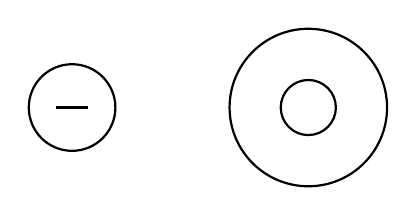
\begin{tikzpicture}[scale=1.0]
\draw[thick] (0,0) circle (0.55);
\draw[thick] (3,0) circle (1.0);
\draw[thick] (3,0) circle (0.35);
\draw[thick] (-0.2,0) -- (0.2,0);
\end{tikzpicture}
\end{center}

% ============================================================
\section{\blue{GPU $\rightarrow$ SM $\rightarrow$ Partitions $\rightarrow$ Units (your hierarchy sketch)}}

\subsection*{\blue{Your labeled chain}}
GPU $\downarrow$ (1)\\
SM $\downarrow$ (2)\\
main units (3)

\subsection*{\blue{Your SM partition sketch (recreated)}}
\begin{center}
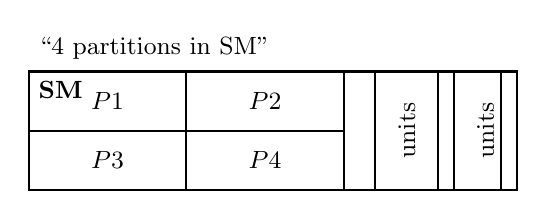
\begin{tikzpicture}[font=\small]
\node[anchor=west] at (0,1.8) {``4 partitions in SM''};

\draw[thick] (0,0) rectangle (6,1.5);
\node[anchor=north west] at (0,1.5) {\textbf{SM}};

\draw[thick] (0,0.75) -- (4,0.75);
\draw[thick] (2,0) -- (2,1.5);
\draw[thick] (4,0) -- (4,1.5);

\node at (1,1.125) {$P1$};
\node at (3,1.125) {$P2$};
\node at (1,0.375) {$P3$};
\node at (3,0.375) {$P4$};

\draw[thick] (4.4,0) rectangle (5.2,1.5);
\draw[thick] (5.4,0) rectangle (6.2,1.5);
\node[rotate=90] at (4.8,0.75) {\small units};
\node[rotate=90] at (5.8,0.75) {\small units};
\end{tikzpicture}
\end{center}

\subsection*{\blue{You listed these parts}}
\begin{enumerate}
\item L0 cache $\rightarrow$ 4
\item 32 thread in a warp $\Rightarrow$ \textbf{SIMT}
\item warp scheduler
\item dispatcher unit
\item register files
\item computational units
\end{enumerate}

\begin{bluebox}
\textbf{Memory recall:} \\
\textbf{Scheduler} picks \emph{which warp} runs; \textbf{dispatcher} issues the instruction to the pipelines/cores.
\end{bluebox}

% ============================================================
\section{\blue{Tensor core perf / architecture + CUDA toolchain}}

You wrote:
\begin{itemize}
\item Tensor core perf can vary based on arch (ex. Volta vs Ampere)
\item It is possible that FP16 product can be FP32 (depending on the arch)
\item GPUs have max threads depending on the arch
\item NVLink vs PCIe
\end{itemize}

\subsection*{\blue{CUDA toolchain (your notes)}}
CUDA $\Rightarrow$ compute unified device arch\\
CUDA compiler = NVCC
\begin{itemize}
\item transforms CUDA to HW PTX code
\item then obtains an executable file
\end{itemize}

\subsection*{\blue{CUDA libraries (your notes)}}
CUDA libraries:
\begin{itemize}
\item cuBLAS $\Rightarrow$ GPU accelerated linear alg
\item cuFFT $\Rightarrow$ fast fourier transform library
\item cuDNN $\Rightarrow$ DNN used for deep learning acceleration
\end{itemize}

\subsection*{\blue{CUDA runtime + driver APIs (your notes)}}
CUDA runtime + driver APIs:
\begin{itemize}
\item managing devices, mem, program exec on GPU
\item \texttt{cudaMalloc()} allocate mem \quad ($\rightarrow$ plain malloc() is just on CPU)
\item \texttt{cudaMemcpy()} \quad ($\rightarrow$ copying data GPU $\leftrightarrow$ CPU)
\end{itemize}

\subsection*{\blue{Tools for debugging + perf analysis (your notes)}}
\begin{itemize}
\item Nsight systems $\Rightarrow$ system wide perf \quad ($\rightarrow$ compute: kernel profiling)
\item CUDA GDB $\Rightarrow$ debugging CUDA
\item cuda memcheck $\Rightarrow$ memory errors
\end{itemize}

\subsection*{\blue{Table: Quick “which tool for what?”}}
\begin{center}
\renewcommand{\arraystretch}{1.15}
\begin{tabular}{|>{\bfseries}p{0.22\linewidth}|p{0.72\linewidth}|}
\hline
Tool & Best for \\
\hline
Nsight Systems & End-to-end timeline: CPU+GPU overlap, launches, syncs, memcpy \\
\hline
Nsight Compute & Deep kernel analysis: occupancy, memory throughput, instruction mix \\
\hline
cuda-gdb & Debugging kernels (breakpoints, stepping) \\
\hline
cuda-memcheck & Memory correctness (OOB, race-ish issues, leaks) \\
\hline
\end{tabular}
\end{center}

% ============================================================
\section{\blue{Mapping SW from CPU to HW (your diagrams)}}

\textbf{Mapping SW from CPU to HW}
\begin{itemize}
\item GPGPU $\Rightarrow$ general purpose on GPU
\item Based on C, compiler NVCC (but is not just a compiler help use GPU resources)
\end{itemize}

\subsection*{\blue{Your CPU/GPU + DRAM + PCIe sketch (recreated)}}
\begin{center}
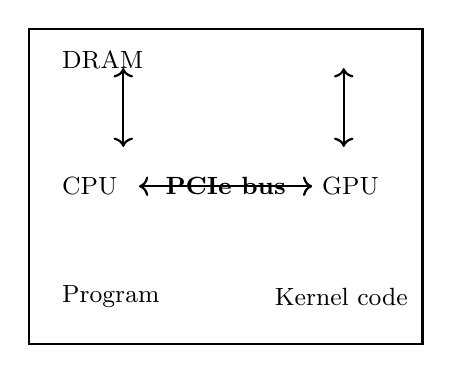
\begin{tikzpicture}[font=\small]
\draw[thick] (0,0) rectangle (5,4);

\node[anchor=west] at (0.3,3.6) {DRAM};
\node[anchor=west] at (0.3,2.0) {CPU};
\node[anchor=west] at (3.6,2.0) {GPU};

\draw[<->, thick] (1.2,3.5) -- (1.2,2.5);
\draw[<->, thick] (4.0,3.5) -- (4.0,2.5);

\node at (2.5,2.0) {\textbf{PCIe bus}};
\draw[<->, thick] (1.4,2.0) -- (3.6,2.0);

\node[anchor=west] at (0.3,0.6) {Program};
\node[anchor=west] at (3.0,0.6) {Kernel code};
\end{tikzpicture}
\end{center}

\subsection*{\blue{Your “GPU has 4 levels of hierarchy / SM 2 level / partitions / core”}}
\begin{enumerate}
\item GPU $\rightarrow$ 4 levels of hierarchy
\item SM in 2 level \\
\quad each SM is divided in partitions (level 3) \\
\quad SM has 4 partitions
\item FP32 core
\end{enumerate}

So we need to understand how each part program maps to the different levels of GPU using threads or blocks.

\subsection*{\blue{Visualization: Grid $\rightarrow$ Blocks $\rightarrow$ SMs}}
\begin{center}
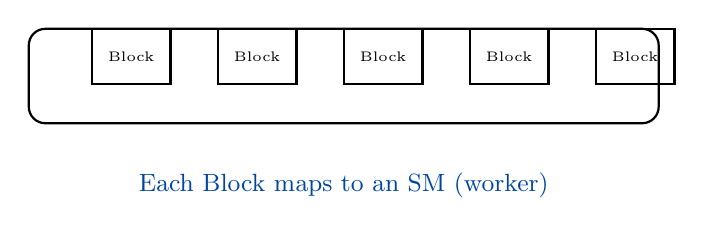
\begin{tikzpicture}[font=\small, node distance=10pt]
\node[draw, thick, rounded corners=6pt, minimum width=8cm, minimum height=1.2cm, align=center] (grid) {};
\foreach \x in {-3.2,-1.6,0,1.6,3.2}{
  \draw[thick] ($(grid.center)+(\x,-0.1)$) rectangle ++(1.0,0.7);
  \node at ($(grid.center)+(\x+0.5,0.25)$) {\tiny Block};
}
\node[below=14pt of grid] (note) {\blue{Each Block maps to an SM (worker)}};
\end{tikzpicture}
\end{center}

% ============================================================
\section{\blue{Blocks, warps, scheduling, dispatch (your “level 2/3” notes)}}

\textbf{Block} $\rightarrow$ think of each block of tasks (job)\\
\quad which is sent to a SM (worker)

So who is the manager coordinating jobs $\Leftrightarrow$ workers?\\
\textbf{the GIGATHREAD} \red{(level 2!!)}\\
\quad $\Rightarrow$ thread is connected to all SMs!

\begin{redbox}
\textbf{But... how do we deal with the SM partitions?}\\
can't just assign to one partition and leave other 3 partitions
\end{redbox}

So... blocks further division into warps will allow us to divide into the four partitions.

\subsection*{\blue{Your “what happens when we $\uparrow$ \# of warps”}}
What happens when we $\uparrow$ \# of warps \red{(level 3)}\\
we have a \textbf{warp scheduler} for scheduling each warp for each cycle

So what happens in each core?\\
warp $\rightarrow$ 32 threads \\
A \textbf{DISPATCHER} makes sure that every core in the partition is actively engaged in the computational process

\subsection*{\blue{Small diagram: Block split into Warps}}
\begin{center}
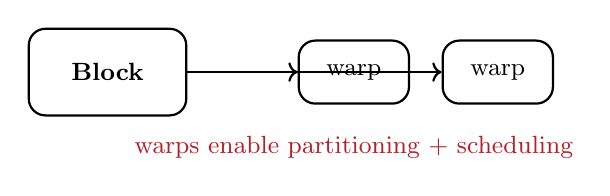
\begin{tikzpicture}[font=\small]
\node[draw, thick, rounded corners=6pt, minimum width=2.0cm, minimum height=1.1cm] (block) {\textbf{Block}};
\node[draw, thick, rounded corners=6pt, minimum width=1.4cm, minimum height=0.8cm, right=1.4cm of block] (w1) {warp};
\node[draw, thick, rounded corners=6pt, minimum width=1.4cm, minimum height=0.8cm, right=0.4cm of w1] (w2) {warp};
\draw[->, thick] (block) -- (w1);
\draw[->, thick] (block) -- (w2);
\node[below=8pt of w1] {\red{warps enable partitioning + scheduling}};
\end{tikzpicture}
\end{center}

\subsection*{\blue{Your summary (preserved)}}
\textbf{SUMMARY}
\begin{enumerate}
\item GPU
\item SM \quad (block / giga threads)
\item partition \quad (warp / warp scheduler)
\item core \quad (thread / dispatcher)
\end{enumerate}

% ============================================================
\section{\blue{Need to specify \# of threads and \# of blocks (your occupancy notes)}}

Need to specify \# of threads and \# of blocks\\
For warps? Divide block size \#threads/blocks by 32\\
Warps are fixed and are \red{32 threads}

\subsection*{\blue{Volta arch (your limits)}}
Volta arch:
\begin{itemize}
\item max threads per block = 1024
\item max threads per SM = 2048
\end{itemize}

So... think like this:
\begin{itemize}
\item 1024 threads/block = max 2 blocks per SM
\item 512 $\rightarrow$ 4 blocks
\item 256 $\rightarrow$ 8 blocks
\end{itemize}

SM must be busy every cycle!\\
$\Rightarrow$ if 1 warp stalls, SM needs to make another warp ready = \red{Latency Hiding}\\
but... how many regs + shared mem a block uses can effect

\subsection*{\blue{Large Blocks}}
\textbf{Large Blocks}
\begin{enumerate}
\item more thread can share shared mem \checkmark
\item fewer redundant global mem loads \checkmark
\item easier reductions, tiling, reuse \checkmark
\end{enumerate}
\textbf{Better data sharing + coordination}

\red{$\downarrow$ If 2 blocks per SM then if 1 block stalls?}\\
$\Rightarrow$ fewer active warps $\Rightarrow$ less latency hiding\\
\red{$\downarrow$ occupancy drops} $\Rightarrow$ \blue{not bad} but... \red{$\downarrow$ flexibility}

Occupancy = active warps / max possible warps\\
bc of more reg/shared mem per thread $\Rightarrow$ $\downarrow$ \# of blocks per SM $\Rightarrow$ $\downarrow$ active warps

\subsection*{\blue{Small Blocks}}
\textbf{Small Blocks}
\begin{enumerate}
\item more blocks $\rightarrow$ more warps $\rightarrow$ better latency hiding \checkmark
\end{enumerate}
\quad fit more easily on SM $\uparrow$ pool of runnable warps

\red{$\downarrow$ less coordination + reuse}
\begin{enumerate}
\item fewer threads cooperating
\item smaller shared mem tiles
\item more global mem traffic
\end{enumerate}

What does this mean?
\begin{enumerate}
\item $\uparrow$ mem bandwidth usage
\item $\downarrow$ reduce arithmetic intensity
\item hurt cache locality
\end{enumerate}
Basically... may be loading data mult times

\subsection*{\blue{Table: Large vs Small blocks (memory recall)}}
\begin{center}
\renewcommand{\arraystretch}{1.15}
\begin{tabular}{|>{\bfseries}p{0.22\linewidth}|p{0.36\linewidth}|p{0.36\linewidth}|}
\hline
 & Large blocks & Small blocks \\
\hline
Reuse / shared memory & \blue{Higher} (good tiling) & \red{Lower} \\
\hline
Latency hiding & \red{Can be worse} if fewer warps & \blue{Often better} (more runnable warps) \\
\hline
Global memory traffic & \blue{Often lower} & \red{Often higher} \\
\hline
Occupancy & \red{May drop} (regs/shmem limit) & \blue{May rise} (more blocks fit) \\
\hline
\end{tabular}
\end{center}

\begin{redbox}
\textbf{Important:} High occupancy is a tool for \emph{latency hiding}, not a guarantee of max performance.
\end{redbox}

% ============================================================
\section{\blue{Vector size / chunking notes (your “8x smaller chunk” idea)}}

Large $\#'s$ continued: remember when you change vector size change config of application\\
remember mult by 4 to get total of \# of bytes

\[
\#\texttt{define SIZE } 1024\cdot 1024\cdot 128
\]
need a
\[
\#\texttt{define CHUNK : smaller vector chunks : } 1024\cdot 1024\cdot 1024
\]

8x smaller chunk, doing each piece sequentially\\
use a for loop to iterate over the 8 chunks\\
$\uparrow$ this process of using chunks reduces the mem being used at a certain time

\subsection*{\blue{Visualization: Chunking timeline}}
\begin{center}
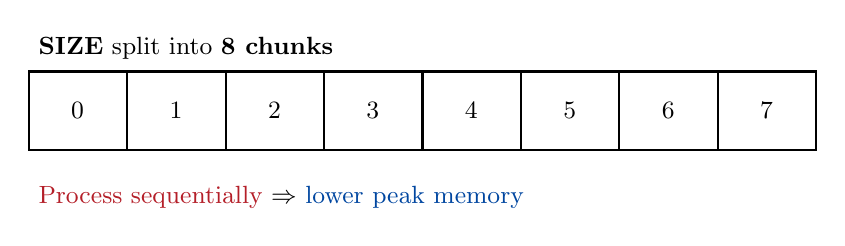
\begin{tikzpicture}[font=\small]
\draw[thick] (0,0) rectangle (10,1);
\node[anchor=west] at (0,1.3) {\textbf{SIZE} split into \textbf{8 chunks}};
\foreach \i in {0,...,7} {
  \draw[thick] (1.25*\i,0) -- (1.25*\i,1);
  \node at (1.25*\i+0.62,0.5) {\i};
}
\node[anchor=west] at (0,-0.6) {\red{Process sequentially} $\Rightarrow$ \blue{lower peak memory}};
\end{tikzpicture}
\end{center}

% ============================================================
\section{\blue{Extra quick “memory recall” tables}}

\subsection*{\blue{Table: Vocabulary mapping (CPU analogy)}}
\begin{center}
\renewcommand{\arraystretch}{1.15}
\begin{tabular}{|>{\bfseries}p{0.24\linewidth}|p{0.68\linewidth}|}
\hline
Term & Meaning (in your words) \\
\hline
Block & block of tasks (job) sent to an SM (worker) \\
\hline
Warp & fixed group of \red{32 threads} (SIMT unit) \\
\hline
Warp scheduler & schedules each warp for each cycle \\
\hline
Dispatcher & keeps cores engaged / issues work into partition pipelines \\
\hline
GigaThread engine & manager coordinating blocks across SMs (\red{level 2!!}) \\
\hline
\end{tabular}
\end{center}

\subsection*{\blue{Table: Perf drivers you listed (fast checklist)}}
\begin{center}
\renewcommand{\arraystretch}{1.15}
\begin{tabular}{|>{\bfseries}p{0.25\linewidth}|p{0.67\linewidth}|}
\hline
Driver & What to ask yourself \\
\hline
Memory bandwidth & Is this kernel waiting on memory? Are loads coalesced? \\
\hline
TFLOPS & Is the kernel compute-heavy and using the right math units? \\
\hline
Tensor cores & Can I use FP16/BF16/TF32 + matrix ops to hit tensor cores? \\
\hline
Occupancy & Do regs/shmem limit active warps and reduce latency hiding? \\
\hline
\end{tabular}
\end{center}

% ============================================================
% ============================================================
\section{Runtime API Functions}

\begin{bluebox}
\textbf{Goal of this section:} use CUDA \textbf{runtime API} calls to \textbf{query the GPU(s)} on your system and understand key hardware limits (threads, grid dims, bandwidth, SM count, CC).
\end{bluebox}

\noindent\texttt{cudaGetDeviceCount(\&nDevices);} \\
\noindent \textit{Runtime API function that gets the number of CUDA-capable devices on the system. It stores the total number of GPUs in \texttt{nDevices}.}

\medskip
\noindent\texttt{cudaGetDeviceProperties(\&prop, i);} \\
\noindent \textit{Use this in a loop for all devices listed (i = 0 to nDevices-1) to query each GPU’s properties.}

\subsection*{\blue{Example output (device query)}}
You get something like:

\begin{verbatim}
Device Number: 0
Device name: Tesla V100-PCIE-32GB
Memory Clock Rate (KHz): 877000
Memory Bus Width (bits): 4096
Peak Memory Bandwidth (GB/s): 898.048000

Total global memory: 34072559616 : 34 gb
Compute capability: 7.0
Number of SMs: 80
Max threads per block: 1024
\end{verbatim}

\begin{bluebox}
\textbf{Memory recall:} Peak memory bandwidth is \textbf{roughly} derived from memory clock + bus width.\\
\textbf{Idea:} wider bus and faster memory clock $\Rightarrow$ more bytes/sec $\Rightarrow$ potentially better throughput for memory-bound kernels.
\end{bluebox}

\subsection*{\blue{Warp note (preserved)}}
\noindent\texttt{// NOTES each WARP is 32 so WARP = 32}

\begin{redbox}
\textbf{Warp = 32 threads} is a \textbf{hardware scheduling unit} in NVIDIA GPUs (SIMT). Many performance concepts (like occupancy + latency hiding) depend on how many \textbf{warps} are active.
\end{redbox}

\subsection*{\blue{Occupancy (INSERT filled): what is it and why important?}}
\textbf{Occupancy} is the fraction of the maximum possible number of \textbf{active warps} on an SM that your kernel actually has active:
\[
\textbf{Occupancy}=\frac{\text{active warps per SM}}{\text{max warps per SM}}
\]

\begin{itemize}
\item \blue{\textbf{Why it matters:}} Occupancy helps \red{\textbf{hide latency}}. When one warp stalls (memory, dependency), the SM can switch to another ready warp.
\item \red{\textbf{What it does NOT guarantee:}} High occupancy does \textbf{not automatically mean fast}. If you’re memory-bandwidth limited, more warps may not help.
\end{itemize}

\subsection*{\blue{Max thread dimensions (INSERT filled): what does this mean simply?}}
\noindent\texttt{Max threads dimensions: x = 1024, y = 1024, z = 64}

\begin{bluebox}
\textbf{Simple meaning:} this is the \textbf{maximum size of a CUDA block} in each dimension.\\
You can launch a block as \texttt{dim3(blockX, blockY, blockZ)} but each axis has a limit.\\
Also, \textbf{total threads per block} is still limited (e.g., \textbf{1024} threads total on V100).
\end{bluebox}

\subsection*{\blue{Max grid dimensions (INSERT filled): what does this mean simply?}}
\noindent\texttt{Max grid dimensions: x = 2147483647, y = 65535, z = 65535}

\begin{bluebox}
\textbf{Simple meaning:} this is the maximum number of \textbf{blocks in the grid} you can launch along each axis.\\
Grid size = \texttt{dim3(gridX, gridY, gridZ)}. This controls how many blocks exist overall.
\end{bluebox}

\subsection*{\blue{Visualization: Thread hierarchy (grid $\rightarrow$ block $\rightarrow$ warp)}}
\begin{center}
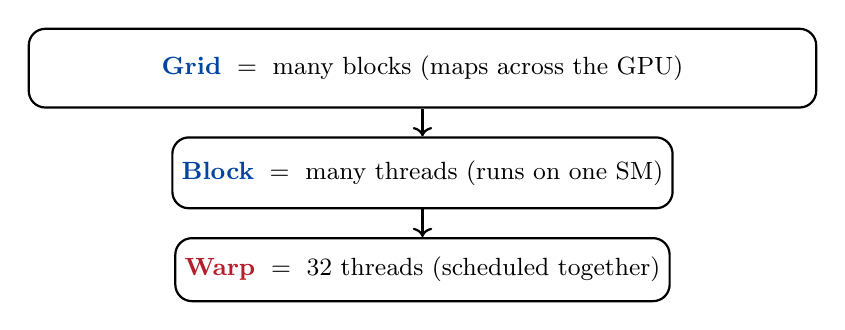
\begin{tikzpicture}[font=\small, node distance=10pt]
\node[draw, rounded corners=6pt, thick, minimum width=10cm, minimum height=1cm, align=center] (grid)
{\blue{\textbf{Grid}} \;=\; many blocks (maps across the GPU)};
\node[draw, rounded corners=6pt, thick, below=10pt of grid, minimum width=6cm, minimum height=0.9cm, align=center] (block)
{\blue{\textbf{Block}} \;=\; many threads (runs on one SM)};
\node[draw, rounded corners=6pt, thick, below=10pt of block, minimum width=4cm, minimum height=0.8cm, align=center] (warp)
{\red{\textbf{Warp}} \;=\; 32 threads (scheduled together)};
\draw[->, thick] (grid) -- (block);
\draw[->, thick] (block) -- (warp);
\end{tikzpicture}
\end{center}

% ============================================================
\section{NVIDIA-SMI \texorpdfstring{$\rightarrow$}{->} System Management Interface}

\begin{bluebox}
\textbf{What is NVIDIA-SMI?} A command-line tool to \blue{\textbf{monitor}}, \red{\textbf{control}}, and \textbf{query} NVIDIA GPU state.
\end{bluebox}

\subsection*{\blue{Three key features (cleaned + preserved)}}
\begin{itemize}
\item \blue{\textbf{Performance monitoring:}} utilization, memory usage, temperature, and power
\item \red{\textbf{Settings management:}} controlling clock speeds and power limits
\item \textbf{Device info + query:} GPU name, driver version, CUDA version, MIG status, ECC, etc.
\end{itemize}

\subsection*{\blue{Example output (INSERT filled: color coding by feature)}}
\begin{redbox}
\textbf{Color guide for reading the output:}\\
\blue{Blue} = monitoring metrics (util/temp/mem/power) \quad
\red{Red} = settings/limits (P-states, power caps) \quad
\textbf{Black} = device identity + versions
\end{redbox}

\begin{verbatim}
nvidia-smi
Sat Feb  7 23:27:50 2026
+-----------------------------------------------------------------------------------------+
| NVIDIA-SMI 580.105.08             Driver Version: 580.105.08     CUDA Version: 13.0     |
+-----------------------------------------+------------------------+----------------------+
| GPU  Name                 Persistence-M | Bus-Id          Disp.A | Volatile Uncorr. ECC |
| Fan  Temp   Perf          Pwr:Usage/Cap |           Memory-Usage | GPU-Util  Compute M. |
|                                         |                        |               MIG M. |
|=========================================+========================+======================|
|   0  Tesla V100-PCIE-32GB           On  |   00000000:D8:00.0 Off |                    0 |
| N/A   28C    P0             26W /  250W |       0MiB /  32768MiB |      0%      Default |
|                                         |                        |                  N/A |
+-----------------------------------------+------------------------+----------------------+

+-----------------------------------------------------------------------------------------+
| Processes:                                                                              |
|  GPU   GI   CI              PID   Type   Process name                        GPU Memory |
|        ID   ID                                                               Usage      |
|=========================================================================================|
|  No running processes found                                                             |
+-----------------------------------------------------------------------------------------+
\end{verbatim}

\begin{bluebox}
\textbf{Why show driver + CUDA versions?}\\
Some libraries depend on a minimum (or specific) \textbf{driver version} and \textbf{CUDA version}. If something fails to load, checking these is step 1.
\end{bluebox}

\subsection*{\blue{Monitoring GPU continuously (cleaned)}}
Monitoring GPU continuously (Linux command): \texttt{nvidia-smi -l}\\
\textit{This refreshes output every second so you can see GPU util + memory change live.}

\subsection*{\blue{INSERT: useful nvidia-smi commands (filled)}}

\begin{center}
\renewcommand{\arraystretch}{1.15}
\begin{tabular}{|p{0.34\linewidth}|p{0.58\linewidth}|}
\hline
\textbf{Goal} & \textbf{Command} \\
\hline
Show summary (default view) & \texttt{nvidia-smi} \\
\hline
Refresh every 1s & \texttt{nvidia-smi -l 1} \\
\hline
Show specific fields (custom query) &
\texttt{nvidia-smi --query-gpu=name,uuid,utilization.gpu,utilization.memory,temperature.gpu,power.draw,memory.used,memory.total --format=csv} \\
\hline
Save output to a file &
\texttt{nvidia-smi -q > smi\_report.txt} \\
\hline
Check clocks in use (graphics/SM/mem) &
\texttt{nvidia-smi -q -d CLOCK} \\
\hline
Check all supported clocks &
\texttt{nvidia-smi -q -d SUPPORTED\_CLOCKS} \\
\hline
Set power limit (requires permission) &
\texttt{sudo nvidia-smi -pl 200} \\
\hline
Set application clocks (if supported + permitted) &
\texttt{sudo nvidia-smi -ac <memClockMHz>,<smClockMHz>} \\
\hline
Permission note (why it might fail) &
\textbf{If you get “Insufficient Permissions”, you need admin or cluster policy support.} \\
\hline
\end{tabular}
\end{center}

\begin{redbox}
\textbf{Cluster reality:} On shared HPC systems, power/clock changes are often disabled for users. You can still \blue{monitor} everything.
\end{redbox}

% ============================================================
\section{GPU Occupancy and Utilization}

\subsection*{\blue{Theoretical vs achieved occupancy (fixed spelling, preserved meaning)}}
There’s a difference between \textbf{achieved occupancy} and \textbf{theoretical occupancy}:

\begin{itemize}
\item \blue{\textbf{Theoretical occupancy (ideal):}}
calculated as \textit{warps used in kernel} / \textit{max warps per SM}.\\
It refers to the maximum percentage of compute resources a kernel \textbf{could} use under ideal conditions (no bottlenecks: memory, compute dependencies, synchronization).
\item \red{\textbf{Achieved occupancy (actual):}}
what the kernel \textbf{really gets} at runtime. Achieved occupancy is affected by scheduling overhead, imbalance across warps/blocks, stalls, and resource limits (registers/shared memory).
\end{itemize}

\subsection*{\blue{Your mental model (preserved + clarified)}}
Achieved: actual usage. Since GPUs are made of SMs, each SM has multiple partitions. A block runs on an SM, and warps execute on the partition.

\begin{bluebox}
\textbf{Helpful framing:}\\
\textbf{Warps} = software execution groups \quad \textbf{Partitions} = hardware execution lanes\\
Scheduler picks which warp runs; dispatcher issues its instructions.
\end{bluebox}

Each partition has a \textbf{scheduler} that allocates a warp to execute each cycle.\\
A \textbf{dispatcher unit} takes ready instructions and sends them to the appropriate computation units.

\subsection*{\blue{Stalls + latency hiding (fixed grammar, preserved content)}}
There are examples where warps are not ready. A warp can stall anywhere from \textbf{30 to 300 cycles}. During this wait, another warp may run.

However, if there are a lot of memory requests or scheduling dependencies, there are situations where \textbf{no warp can be issued} — this is a \red{\textbf{STALL cycle}}.

\begin{redbox}
\textbf{Latency hiding:} the whole point of having many warps is that when one stalls, another runs.\\
If \textbf{all} warps stall, you get visible idle cycles.
\end{redbox} 



\subsection*{\blue{Your NVBit note (preserved, clarified)}}
Scenario: (1) no memory dependency / dependency.\\
NVBit: assembly is SASS instructions.

We are able to see the software for each warp in assembly, and observe what warps are doing.

Say you have four warps on one partition: \\
How many warps are utilized per partition? \\
In this case you can see there is 


#warps/p = 4 warps
#arps/sm = 4*4=16 warps

say you ha ve the assembly code,  
warm schduel chooses one of the warps to excuted

ex) a flop instruction , warp sheduleder says i have warp 0 and its ready then the dispatcher with thake the first intrsuction here and send it to al the core heres that are FP32, 

so ii its once instrc why is it sent to all fp32? thats because each warp is 32 threads but on diffrent data, so each assemply linea fter the first istruct it will be sent to all the core with idffrent reg,

in the next cylce, scheduler as the warps which one is ready
goes into the cycle into each warp,




% ============================================================
\section{Profiling with NCU (Nsight Compute) — vecAdd example}

\begin{bluebox}
\textbf{Goal:} If you run a file, you can profile the app with \textbf{NCU} to understand whether you are compute-bound or memory-bound, and to see occupancy + launch stats.
\end{bluebox}

So if you run a file, all you need to do is profile the app. You can use the command:

\begin{verbatim}
ncu ./vecAdd
\end{verbatim}

\subsection*{\blue{Example output (cleaned, preserved)}}
\begin{verbatim}
==PROF== Profiling "vecAdd" - 0: 0%
==WARNING== Backing up device memory in system memory. Kernel replay might be slow.
           Consider using "--replay-mode application" to avoid memory save-and-restore.
....50%....100% - 19 passes
Execution time: 4944.171387 ms

Finished
==PROF== Disconnected from process 1141543
[1141543] vectorAdd@127.0.0.1
  vecAdd(int *, int *, int *, int) (442368, 1, 1)x(1024, 1, 1), Context 1, Stream 7, Device 0, CC 7.0
\end{verbatim}

\begin{redbox}
\textbf{INSERT filled: total number of blocks}\\
Grid size \texttt{(442368, 1, 1)} means \red{\textbf{442,368 blocks total}} are launched (in X dimension).
\end{redbox}

\subsection*{\blue{Visualization: Launch configuration}}
\begin{center}
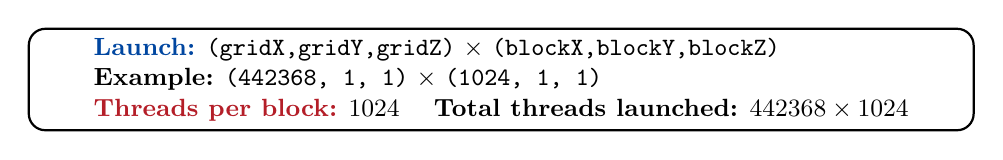
\begin{tikzpicture}[font=\small]
\node[draw, rounded corners=6pt, thick, align=left, minimum width=12cm] (cfg) {
\blue{\textbf{Launch:}} \texttt{(gridX,gridY,gridZ)} $\times$ \texttt{(blockX,blockY,blockZ)}\\
\textbf{Example:} \texttt{(442368, 1, 1)} $\times$ \texttt{(1024, 1, 1)}\\
\red{\textbf{Threads per block:}} $1024$ \quad \textbf{Total threads launched:} $442368 \times 1024$
};
\end{tikzpicture}
\end{center}

\subsection*{\blue{GPU Speed Of Light Throughput (table version)}}
\begin{center}
\renewcommand{\arraystretch}{1.15}
\begin{tabular}{|p{0.48\linewidth}|p{0.20\linewidth}|p{0.22\linewidth}|}
\hline
\textbf{Metric Name} & \textbf{Unit} & \textbf{Value} \\
\hline
DRAM Frequency & MHz & 876.40 \\
\hline
SM Frequency & GHz & 1.24 \\
\hline
Elapsed Cycles & cycles & 8,215,186 \\
\hline
\blue{Memory Throughput} & \% & 91.11 \\
\hline
\blue{DRAM Throughput} & \% & 91.11 \\
\hline
Duration & ms & 6.65 \\
\hline
L1/TEX Cache Throughput & \% & 25.88 \\
\hline
L2 Cache Throughput & \% & 34.03 \\
\hline
SM Active Cycles & cycles & 8,159,381 \\
\hline
\red{Compute (SM) Throughput} & \% & 10.78 \\
\hline
\end{tabular}
\end{center}

\begin{redbox}
\textbf{Quick read:} Memory throughput is \blue{\textbf{very high}} (91\%) while compute throughput is \red{\textbf{low}} (10.78\%).\\
This strongly suggests the kernel is \blue{\textbf{memory-bound}} (DRAM is the limiter).
\end{redbox}

\subsection*{\blue{Launch Statistics (table version)}}
\begin{center}
\renewcommand{\arraystretch}{1.15}
\begin{tabular}{|p{0.55\linewidth}|p{0.35\linewidth}|}
\hline
\textbf{Metric} & \textbf{Value} \\
\hline
Block Size & 1024 \\
\hline
Grid Size & 442368 \\
\hline
Registers Per Thread & 16 \\
\hline
Static Shared Memory Per Block & 0 bytes \\
\hline
Dynamic Shared Memory Per Block & 0 bytes \\
\hline
\# SMs & 80 \\
\hline
Threads (total) & 452,984,832 \\
\hline
Waves Per SM & 2764.80 \\
\hline
\end{tabular}
\end{center}

\subsection*{\blue{Occupancy section (preserved + clarified + extra table)}}
\textbf{Section: Occupancy} // here is what we are looking at:

\begin{center}
\renewcommand{\arraystretch}{1.15}
\begin{tabular}{|p{0.55\linewidth}|p{0.35\linewidth}|}
\hline
\textbf{Metric Name} & \textbf{Metric Value} \\
\hline
Block Limit SM & 32 \\
\hline
Block Limit Registers & 4 \\
\hline
Block Limit Shared Mem & 32 \\
\hline
Block Limit Warps & 2 \\
\hline
Theoretical Active Warps per SM & 64 \\
\hline
Theoretical Occupancy & 100\% \\
\hline
Achieved Occupancy & \red{83.02\%} \\
\hline
Achieved Active Warps Per SM & 53.13 \\
\hline
\end{tabular}
\end{center}

\begin{bluebox}
\textbf{Memory recall: why achieved < theoretical?}\\
Even if resources allow 100\% occupancy, real execution can be lower due to:
warp scheduling overhead, uneven work distribution, divergence, or stalls.
\end{bluebox}

\noindent \textit{Your note (cleaned, preserved):} We are using a good amount, but the number of threads can affect the occupancy of your application. Changing the number of threads per block can change occupancy. We are going to execute 32 blocks simultaneously per SM. Let’s take this value, and calculate theoretical occupancy and get a percentage.

\begin{redbox}
\textbf{Important clarification:}\\
Occupancy is \textbf{not} “blocks per SM”. It is \textbf{active warps per SM} divided by max warps per SM.\\
Blocks per SM influences occupancy because each block contributes warps, but registers/shared memory can cap blocks and warps.
\end{redbox}

\subsection*{\blue{GPU + Memory Workload Distribution (table version)}}
\begin{center}
\renewcommand{\arraystretch}{1.15}
\begin{tabular}{|p{0.52\linewidth}|p{0.38\linewidth}|}
\hline
\textbf{Metric Name} & \textbf{Metric Value} \\
\hline
Average DRAM Active Cycles & 5,306,905.59 \\
\hline
Total DRAM Elapsed Cycles & 186,398,080 \\
\hline
Average L1 Active Cycles & 8,159,381 \\
\hline
Total L1 Elapsed Cycles & 656,324,412 \\
\hline
Average L2 Active Cycles & 7,782,946.30 \\
\hline
Total L2 Elapsed Cycles & 499,117,376 \\
\hline
Average SM Active Cycles & 8,159,381 \\
\hline
Total SM Elapsed Cycles & 656,324,412 \\
\hline
Average SMSP Active Cycles & 8,119,229.41 \\
\hline
Total SMSP Elapsed Cycles & 2,625,297,648 \\
\hline
\end{tabular}
\end{center}

\begin{bluebox}
\textbf{Interpretation hint:} If DRAM throughput is high and compute throughput is low, optimize memory behavior first:
coalescing, fewer global loads, more reuse (tiling/shared memory), better cache locality.
\end{bluebox}


\end{document}
